%!TEX root = ../aamas11storage.tex
% %%%%%%%%%%%%%%%%%%%%%%%%%%%%%%%%%%%%%%%%%%%%%%%%%%%
\section{The BDI Learning Framework}\label{sec:framework}
% %%%%%%%%%%%%%%%%%%%%%%%%%%%%%%%%%%%%%%%%%%%%%%%%%%%

We begin by briefly reviewing the basic agent programming framework that will be used throughout the paper~\cite{airiau09:enhancing,singh10:extending,singh10:learning}, which is a seamless integration of standard Belief-Desire-Intention (BDI) agent-oriented programming~\cite{Rao96:AgentSpeak,WooldridgeBook} with decision tree learning~\cite{Mitchell97:ML}. 

Generally speaking, BDI agent-oriented programming languages are built around an explicit representation of propositional attitudes (e.g., beliefs, desires, intentions, etc.). 
%%
There are a plethora of agent programming languages and development platforms in the BDI tradition, including
%such as \PRS\ \cite{Georgeff89-PRS},
\JACK~\cite{BusettaRHL:AL99-JACK}, 
\JADEX~\cite{Pokahr:EXP03-JADEX}, and
%\TAPL~\cite{Hindriks99:Agent} and
%\DAPL~\cite{Dastani:JAAMAS08-2APL}, 
\JASON~\cite{jasonbook}
%, and SRI's \SPARK~\cite{MorelyM:AAMAS04-SPARK}, 
among others. 
%%
A BDI architecture addresses how these components are represented, updated, and processed to determine the agent's actions.
%%
Specifically, a BDI intelligent agent systematically chooses and executes \emph{plans} (i.e., operational procedures) to achieve or realize its goals, called \emph{events}.
%%
Such plans are extracted from the so-called agent's \emph{plan library}, which encode the ``know-how'' information of the domain the agent operates on.
%%
For instance, the plan library of an unmanned air vehicle (UAV) agent controller may include several plans to address the event-goal of landing the aircraft. Each plan is associated with a \emph{context condition} stating under which belief conditions the plan is a sensible strategy for resolving the goal in question. Whereas some plans for landing the aircraft may only be suitable under normal weather conditions, other plans may only be used under emergency operations.
%%%
Besides the actual execution of domain actions (e.g., lifting the flaps), a plan may require the resolution of (intermediate) sub-goal events (e.g., obtain landing permission from air control tower). As a result, the execution of a BDI system can be seen as a \textit{context sensitive subgoal expansion}, allowing agents to ``act as they go'' by making \emph{plan choices} at each level of abstraction with respect to the current situation. The use of plans' context (pre)conditions to make choices as late as possible, together with the built-in goal-failure mechanisms, ensures that the system is responsive to changes in the environment. 

\begin{figure}[t]
\begin{center}
%\resizebox{.45\textwidth}{!}{
%!TEX root = ../ijcai11storage.tex
\begin{tikzpicture}[level distance=1.0cm]
\tikzstyle{succ}=[label=below:$\surd$]
\tikzstyle{fail}=[label=below:$\times$]
\tikzstyle{trace}=[solid,style=circle,fill=black!20,above left=0.15cm,scale=.7]

\tikzstyle{planbox}=[draw,minimum height=0.6cm,minimum width=0.65cm]
\tikzstyle{goalbox}=[draw,minimum height=0.6cm,minimum width=0.65cm,rounded corners=0.2cm]
\tikzstyle{planbox2}=[planbox,pattern=north west lines,pattern color=black!30]
\tikzstyle{goalbox2}=[goalbox,pattern=north west lines,pattern color=black!30]
\tikzstyle{goalbox3}=[goalbox,fill=black!20]
\tikzstyle{planbox3}=[planbox,fill=black!20]

	
\tikzstyle{level 1}=[sibling distance=2.7cm] 
\tikzstyle{level 2}=[sibling distance=0.9cm] 
\tikzstyle{level 3}=[sibling distance=2.7cm]
\tikzstyle{level 4}=[sibling distance=0.9cm]

\node[planbox3,solid] {$P$}
		child {node[goalbox2] {$G_{1}$}
			child {node[planbox2] {$P_{a}$}
				child {node[goalbox2] {$G_{3}$}
					child {node[planbox,fail] {$P_{g}$}}
					child {node[planbox,fail] {$P_{h}$}}
					child {node[planbox2,succ] {$P_{i}$}}
				}
			}
			child {node[planbox,fail] {$P_{b}$}}
			child {node[planbox,fail] {$P_{c}$}}
		}
		child {node[goalbox3] {$G_{2}$}
			child {node[planbox,fail] {$P_{d}$}}
			child {node[planbox,fail] {$P_{e}$}}
			child {node[planbox3] {$P_f$}
				child {node[goalbox2] {$G_{4}$}
					child {node[planbox,fail] {$P_{j}$}}
					child {node[planbox2,succ] {$P_{k}$}}
					child {node[planbox,fail] {$P_{l}$}}
				}
				child {node[goalbox3] {$G_{5}$}
					child {node[planbox3,succ] {$P_{m}$}}
					child {node[planbox,fail] {$P_{n}$}}
					child {node[planbox,fail] {$P_{o}$}}
				}
			}
		}
		
;

\end{tikzpicture}

%}
\end{center}
\caption{An example goal-plan hierarchy.}
\label{fig:confidence}
\end{figure}


It is not hard to see that, by grouping together plans responding to the same event type, the agent's plan library can be seen as
a set of goal-plan tree templates (e.g., Figure~\ref{fig:confidence}): a goal-event node (e.g., goal $G_1$) has children representing the alternative \emph{relevant} plans for achieving it (e.g., $P_a,P_b$ and $P_c$); and a plan node (e.g., $P_f$), in turn, has children nodes representing the subgoals (including primitive actions) of the plan (e.g., $G_4$ and $G_5$). These structures, can be seen as AND/OR trees: for a plan to succeed all the subgoals and actions of the plan must be successful (AND); for a subgoal to succeed one of the plans to achieve it must succeed (OR). Leaf plans are meant to directly interact with the environment and so, in a given world state, they can either succeed or fail when executed; this is marked accordingly in the figure for some particular world (of course such plans may behave differently in other states).


As can be seen, adequate plan selection is critically important in BDI systems. Whereas standard BDI platforms leverage domain expertise by means of the \emph{fixed} logical context conditions of plans, in this work, we are interested in exploring how a situated agent may \emph{learn} or \emph{improve} its plan selection mechanism based on experience, in order to better realize its goals.
%%
To that end, it was proposed to generalize the account for plans' context conditions to decision trees~\cite{Mitchell97:ML} that can be learnt over time~\cite{airiau09:enhancing,singh10:extending,singh10:learning}. The idea is simple: \emph{the decision tree of an agent plan provides a judgement as to whether the plan is likely to succeed or fail for the given situation.}
%%
By suitably \emph{learning} the structure of such decision tree and adequately \emph{using} such decision trees, we expect the agent to be able to improve its performance over time and release the domain modeller to encode ``perfect'' plan preconditions. Note that the classical boolean context conditions provided by the designer could (and generally will) still be used as initial necessary but possibly insufficient requirements for each plan that will be further \emph{refined} over time in the course of trying plans in various world states.


Under the new BDI learning framework, two mechanisms become crucial. First, of course, a principled approach to learning such decision trees based on execution experiences is needed. Second, an adequate plan selection scheme compatible with the new type of plans' preconditions is required.
%%
To select plans based on information in the decision trees, the work reported in \cite{singh10:extending,singh10:learning} used a probabilistic method that chooses a plan based on its believed likelihood of success in the given situation. This approach provides a balance between exploitation (we choose plans with relatively higher success expectations more often), and exploration (we sometimes choose plans with lower success expectation to get better confidence in their believed applicability by trying them in more situations). This balance is important because ongoing learning influences future plan selection, and subsequently whether a good solution is learnt.



When it comes to the learning process, the training set for a given plan's decision tree contains samples of the form $[w, o]$, where $w$ is the world state---a vector of discrete attributes---in which the plan was executed and $o$ is the execution outcome, namely, success or failure. Initially, the training set is empty and grows as the agent tries the plan in various world states and records each execution result. 
%%
Since the decision tree inductive bias is a preference for smaller trees, one expects that the decision tree learnt to be built from only those world attributes that are relevant to the corresponding plan's (real) context condition.
%%
Now, due to the hierarchical nature of the plan-goal hierarchy being executed by the agent (c.f. Figure~\ref{fig:confidence}), it is possible that the failure of a plan (e.g., $P$) is only due to a poor plan selection lower in the hierarchy (e.g., $P_l$ is selected for goal $G_4$).
%%
To deal with this issue, the work in \cite{airiau09:enhancing} uses a plan ``stability" measure to take failures into account only when the agent is sufficiently sure that the failure was not due to poor sub-plan choices. Another approach reported is to adjust the plan selection probability based on some measure of our ``confidence'' in the decision tree~\cite{singh10:learning} which considers the reliability of a plan's decision tree to be proportional to the number of sub-plan choices (or paths below the plan in the goal-plan hierarchy) that have been explored already: the greater the coverage, the more we have explored and the greater the confidence in the resulting decision tree. 

\paragraph{An energy storage domain example}

% Energy storage enables increasing levels of renewable energy in our electricity system, and the rapidly maturing supply chains for several battery technologies encourages electricity utilities, generators, and customers to consider using large battery systems. 



\newcommand{\pSetCharge}{\mathname{SetCharge}}
\newcommand{\pSetDischarge}{\mathname{SetDischarge}}
\newcommand{\pSetNotUsed}{\mathname{SetNotUsed}}
\newcommand{\pExecute}{\mathname{Execute}}

\newcommand{\cSatisfies}{\mathname{sat}}

\newcommand{\aSet}{\mathname{set}}
\newcommand{\aOperate}{\mathname{operate}}
\newcommand{\aEvaluate}{\mathname{evaluate}}

\begin{figure*}[t]
\begin{center}
\subfigure[Use case scenario for a modular battery system.]{\label{fig:usecase}
\resizebox{.9\columnwidth}{!}{%!TEX root = ../aamas11storage.tex
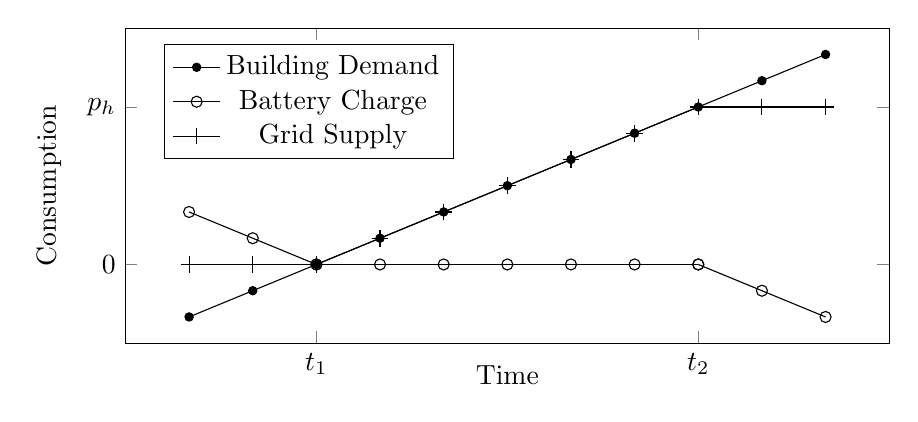
\begin{tikzpicture}

\begin{axis}[
width=0.8\columnwidth,height=4cm,scale only axis,
axis line style={-}, xtick style={-}, ytick style={-},
xlabel=Time,
ylabel=Consumption,
every axis y label/.style={at={(-0.1,0.5)},rotate=90,anchor=center}, 
every axis x label/.style={at={(0.5,-0.1)},anchor=center}, 
%grid=both, grid style={style=densely dotted},
xtick={2,8},
xticklabels={$t_1$,$t_2$},
ytick={0,6},
yticklabels={$0$,$p_h$},
legend style={at={(0.05,0.95)},anchor=north west}
] 

% Draw the Demand-Supply curve
\addplot[-,mark=*,mark size=1.5] expression[domain=0:10,samples=11] {x-2};
\addlegendentry{Building Demand} 

% Draw the Battery curve
\addplot[-,mark=o,mark size=2] expression[forget plot,domain=0:2,samples=3] {2-x}; 
\addplot[-,mark=o,mark size=2] expression[forget plot,domain=2:8,samples=7] {0}; 
\addplot[-,mark=o,mark size=2] expression[domain=8:10,samples=3] {8-x}; 
\addlegendentry{Battery Charge} 

% Draw the Grid supply curve
\addplot[-,mark=+,mark size=3] expression[forget plot,domain=0:2,samples=3] {0}; 
\addplot[-,mark=+,mark size=3] expression[forget plot,domain=2:8,samples=7] {x-2}; 
\addplot[-,mark=+,mark size=3] expression[domain=8:10,samples=3] {6}; 
\addlegendentry{Grid Supply} 
\end{axis} 
\end{tikzpicture} 
}
}
\qquad
\subfigure[Goal-plan hierarchy for a $k$-modules battery system.]{\label{fig:gptree}
\resizebox{.9\columnwidth}{!}{%!TEX root = ../aamas11storage.tex
\begin{tikzpicture} [level distance=8.0em]
\tikzstyle{planbox}=[draw,text width=11.0em,rectangle split,rectangle split parts=3]
\tikzstyle{goalbox}=[draw,rounded corners=1.25em,minimum height=3em,minimum width=5em]

	
\tikzstyle{level 1}=[sibling distance=13.0em] 
\tikzstyle{level 2}=[level distance=7.0em] 

\node[goalbox,solid] {$G($r,k,s$)$}
	child {node[planbox] {$SetCharge$ 
			\nodepart{second} $\psi:satisfies(r,k,s,C),$\\$k>0$
			\nodepart{third} $set(k,C)$
		}
		child {node[goalbox] {$G($r,k-1,s'$)$}}
	}
	child {node[planbox] {$SetDischarge$ \nodepart{second}
			\nodepart{second} $\psi:satisfies(r,k,s,D),$\\$k>0$
			\nodepart{third} $set(k,D)$
		}
		child {node[goalbox] {$G($r,k-1,s'$)$}}
	}
	child {node[planbox] {$SetNotUsed$ \nodepart{second}
			\nodepart{second} $\psi:satisfies(r,k,s,N),$\\$k>0$
			\nodepart{third} $set(k,N)$
		}
		child {node[goalbox] {$G($r,k-1,s'$)$}}
	}
	child {node[planbox] {$Execute$ 
			\nodepart{second} $\psi:k==0$
			\nodepart{third} $operate()$ \\$evaluate()$
		}
	}
;

\end{tikzpicture}


}
}
\caption{An energy storage scenario.}
\end{center}
\label{fig:energystorage}
\end{figure*}



Consider a smart office building comprising of a set of loads (appliances in the building), some renewable sources (solar panels on the roof and a local wind turbine), and a modular battery system. The building is connected to the main grid, and economics govern that the grid power consumption of the building be maintained within the range $[0:p_h]$. 
%%
Since there is little control over the demand in the building and certainly no control over the renewable generation, then for some period in the day it is possible that the power consumption of the building will fall outside this range. For instance, if the renewable generation is high relative to the building loads, then net consumption may fall below $0$. Similarly, if demand is higher than generation then the net building consumption may rise above $p_h$. 
%%
In Figure \ref{fig:usecase} the Building Demand curve for the period prior to $t_1$ and after $t_2$, has this property. While this net demand is fixed for all practical purposes, we do have control over the use of the battery system. By suitably ordering the battery system to charge (act as a load) or discharge (act as a generator) at determined rates through this period we may influence the net demand in the building. Figure \ref{fig:usecase} shows how the appropriate battery response (Battery Charge) added to the net building consumption (Building Demand) ensures that the power drawn from the grid (Grid Supply) is maintained within the desired range.


Large battery systems usually comprise of multiple modules and in many installations these may be controlled independently.  Modules may be operated in synchrony but often there are strategic reasons to keep some modules in a different state to others.  For example, if it is undesirable to change the direction of power flow between charging and discharging too frequently, a subset of modules may be used for each direction until it is necessary to change their roles.  Also, some technologies have specific requirements, such as the zinc-bromine flow battery for which a complete discharge at regular intervals is desirable to ``strip'' the zinc plating and ensure irregularities never have an opportunity to accumulate.  Where they exist these requirements place further constraints on module control.

Given, then, a requested rate of charging and discharging for a large battery installation, we would like a control algorithm for the set of component modules that implements the requested rate as the sum over the module rates of charging and discharging.  While hardwired control of such response is possible, it is not ideal since battery performance is susceptible to change over time and may diverge from normal. What is required is a means of adaptable control that accounts for such drift, and as such, a machine learning approach may be appropriate. 
%The input signal will be different every day but will have many features that are diurnal or nearly so, due to typical variations of electricity demand and solar and wind energy generation sources, and the repetitive patterns that may be seen over several days of the input signal suggest that a learning algorithm may be appropriate.  Our problem is to develop a method for on-line learning that will result in a useful control regime for a modular battery system, when installed at a new site and provided with an input signal derived from the electricity demand and renewable supply at that site.


